\tightsection{Prediction Challenges in Practice}
\label{sec:challenges}

Before we delve into algorithms, we first analyze the challenges of
performing video quality prediction. We first define the main
concepts, and then discuss a method to quantify the lower bound of
prediction error (\Section~\ref{subsec:lowerbound}). Then, we
categorize the factors that cause the prediction error
(\Section~\ref{subsec:challenges}). Based on these understanding, we
propose to aggregate data samples as our basic approach and evaluate
its potential using empirical analysis
(\Section~\ref{subsec:aggregation}).

\tightsubsection{Definitions}
\label{subsec:lowerbound}

\myparatight{Prediction error} 
%We start with defining the {\it prediction error}.  
Given a session (which we will call the {\it session under
  prediction}), let $q$ be the actual quality and $p$ be the predicted
quality\footnote{We consider one quality metric at a time.}. Then, the
{\it prediction error} of this session's quality is $e_{p,q}=|p-q|$.
For a set of sessions under prediction $S=\{s_1,\dots,s_n\}$, let
$P=\{p_i\}$ and $Q=\{q_i\}$ be their predicted and actual qualities,
respectively, where $p_i$ and $q_i$ are the predicted and actual
quality of session $s_i$. Then, we define the overall prediction error
of sessions in $S$ as the square root of the mean square errors:
\begin{align}
&E_{P,Q}=\left(\frac{1}{n}\sum e_{p_i,q_i}^2\right)^{1/2}.
\end{align}

\myparatight{Attribute combination (AC)} An {\it attribute
  combination} ({\it AC}) is simply a set of attributes we use to
characterize the sessions in a given dataset, e.g., $[ASN,
CDN]$. Given AC $g$, a session is represented by its values for all
the attributes in $g$. We say two sessions are {\it g-equivalent}, if
they have identical values for every attribute in $g$. For example, if
$g=[ASN,CDN]$ then all sessions that are connected to the same ASN and
stream data from the same CDN are $g$-equivalent. Thus, $g$ defines a
partition on the set of sessions, where all sessions in a partition
are $g$-equivalent. In addition to the attributes in
\Section~\ref{subsec:dataset}, we also consider temporal
attributes. For instance, given AC $g=[ASN, CDN, 5\,minute]$, two
sessions are $g$-equivalent iff they belong to the same ASN, use the
same CDN and they were streaming during the same 5-minute
interval. The temporal attributes are useful according to previous
research~\cite{sigcomm12} which shows that video quality can vary
significantly over time.

\comment{
Then the attribute combination value of session $s$ on AC $g$, denoted
as $v_g(s)$, is a tuple of values on all attributes in $g$ associated
to $s$. For example, if $g=[ASN,CDN]$ and $s$ is a session from a host
in $ASN1$ that streams video from $CDN1$, $v_g(s)=[ASN1, CDN1]$. We
say two sessions are {\it g-equivalent} with respect to AC $g$, if
they have identical values for every attribute in $g$. Thus, AC $g$
defines a partition on the set of sessions, where all sessions in a
partition are $g$-equivalent. In addition to the attributes in
\Section~\ref{subsec:dataset}, we also consider temporal
attributes. For instance, given AC $g=[ASN, CDN, 5\,minute]$, two
sessions are equivalent iff they belong to the same ASN, use the same
CDN and they were streaming during the same 5-minute interval. The
temporal attributes are useful according to previous
research~\cite{sigcomm12} which shows that video quality can vary
significantly over time.
}

\myparatight{Attribute-based prediction algorithm} An {\it
  attribute-based prediction algorithm} takes a session $s$ (with no
information on its quality) and an AC $g$ as input, and returns the
predicted quality of $s$. Note that such algorithm will make the same
prediction for any two $g$-equivalent sessions.

%This means that if a set of sessions are
%received when the algorithm is given the same AC, their predicted
%qualities only depend on their values on $g$. Specifically, if they
%are equivalent with respect to $g$, they should be given the same
%predicted quality.\jc{some justification to support this assumption.}


\myparatight{Lower bound of prediction error}
%This assumption naturally leads to an {\it lower bound} of prediction error of any algorithm in this kind. 
Given a $g$-equivalent set of sessions $S=\{s_1,\dots,s_n\}$, the
overall prediction error $\left(\frac{1}{n}\sum
  e_{p,q_i}^2\right)^{1/2}$ is minimized when the prediction $p$ for
each of these sessions is equal to the mean of $q_i$, i.e., $p = (\sum
q_i)/n$. More generally, the overall prediction error is minimized
when the \emph{prediction} for sessions in each partition is the mean
of the \emph{actual} quality values of the sessions in that partition.

Intuitively, this lower bound characterizes the dispersion in quality
of the sessions which an AC cannot differentiate. Ideally, if the
attributes selected in AC reflect \emph{all} the factors that
determine the quality of a session, the sessions in the same partition
should produce the same quality and the lower bound is zero. However,
given the measurement limitations and the inherent noises (see
\Section~\ref{subsec:challenges} for detailed discussion), achieving
such lower bound is not trivial in practice.


\tightsubsection{Sources of prediction error}
\label{subsec:challenges}

In general, there are four sources of prediction error:

\begin{packedenumerate}
\item \emph{Estimation error} caused by limited data.  Even other
  things being equal, more data produce more accurate prediction. For
  example, Figure~\ref{fig:group-size-impact} presents the prediction
  error vs. partition size (i.e., number of samples). Given a large number
  of attributes and the combinatorial nature of the attributes (the
  number of partitions grow exponentially with more attributes),
  estimation error is a serious problem in practice.


\begin{figure}[h!]
\centering
\subfigure[Prediction error vs. partition size (w.r.t average bitrate)]
{
        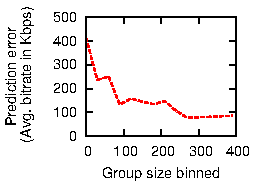
\includegraphics[width=110pt]{figures/count-err.pdf}
	\label{subfig:group-size-impact:count-err}
}
\subfigure[Distribution of partition size]
{
        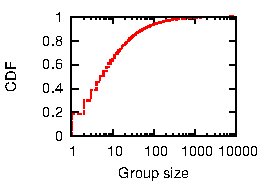
\includegraphics[width=110pt]{figures/count-cdf.pdf}
}
\tightcaption{Impact of partition size (i.e., number of samples in a partition). They show that more samples give more accuracy, but most of partitions do not have sufficient samples for accurate prediction.}
\label{fig:group-size-impact}
\end{figure}

\item \emph{Bias} due to missing or unused information: The bias
  occurs when we do not observe (or use) an attribute that is
  important for prediction. Bias is not alleviated by gathering data
  from more session, but by gathering more attributes from each
  session.

\item \emph{Unavailability of recent data:} In a practical system,
  there are delays in measuring, sending and processing quality
  samples, so they are not available instantly.  If conditions change
  rapidly, there may be no quality samples sufficiently close to the
  session under prediction.  This is an extreme example of estimation
  error.  In this case it may be necessary to model the evolution of
  the video ecosystem over time in order to extrapolate to the current
  time. Figure~\ref{fig:quality-variability} shows per-minute quality
  variability. It shows that even with sufficient data, the mean value
  of quality samples belonging to sessions in the same partition could
  vary significantly. This clearly indicates that any practical
  algorithm has to be running in real-time (on the order of one minute
  or less).

\begin{figure}[h!]
\centering
 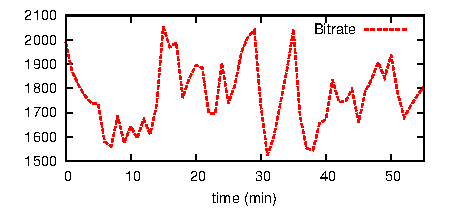
\includegraphics[width=0.4\textwidth] {figures/quality-time.pdf}
\tightcaption{Temporal variability of quality. The figure shows the mean value of average bitrate of a fixed partition of same [Site, Initial CDN, Initial Bitrate, ConnectionType, ASN, Object], which has 100 quality samples in every minute in the figure.}
\label{fig:quality-variability}
\end{figure}

\item \emph{Noise:} Even if we observed all conceivable attributes of
  a session and had infinitely many examples of exactly quality
  samples, outcomes may be affected by non-deterministic inputs.  For
  example, performance may be affected by exponentially backoff at the
  data link layer or the congestion generated by cross traffic at the
  network layer. This implies that some degree of prediction error is
  inevitable.  \xil{can i say this is Bias? because we do not capture
    this feature, and it is hard for us to extract a feature out of
    it, we consider it as noise?}
\end{packedenumerate}

%\jc{In general, we should ack that we cannot address all these challenges. Aggregation only addresses estimation error (or more?) and the rest should be in discussion and future work.}

Thus for any practical algorithm, it is challenging to manage
prediction error, and in some cases even impossible, for examples, if
we have no recent data. Next, we discuss how to address the estimation
error, arguably the main component of prediction error.

\tightsubsection{AC Aggregation and Challenges}
\label{subsec:aggregation}
A simple strategy to reduce estimation error is {\it aggregation}.  By
aggregation we mean using ACs with fewer attributes.  Aggregation
increases the number of samples in each partition, thus reducing
estimation error at the cost of increased bias.  Intuitively, when
estimation error is small (say, when a fine-grained partition contains
many sessions) we want to reduce bias by using a finer grain
partition.  On the other hand, when estimation error is large, we want
to increase the level of aggregation.  Then the question becomes how
to determine the best level of aggregation.


\begin{figure}[h!]
\centering
 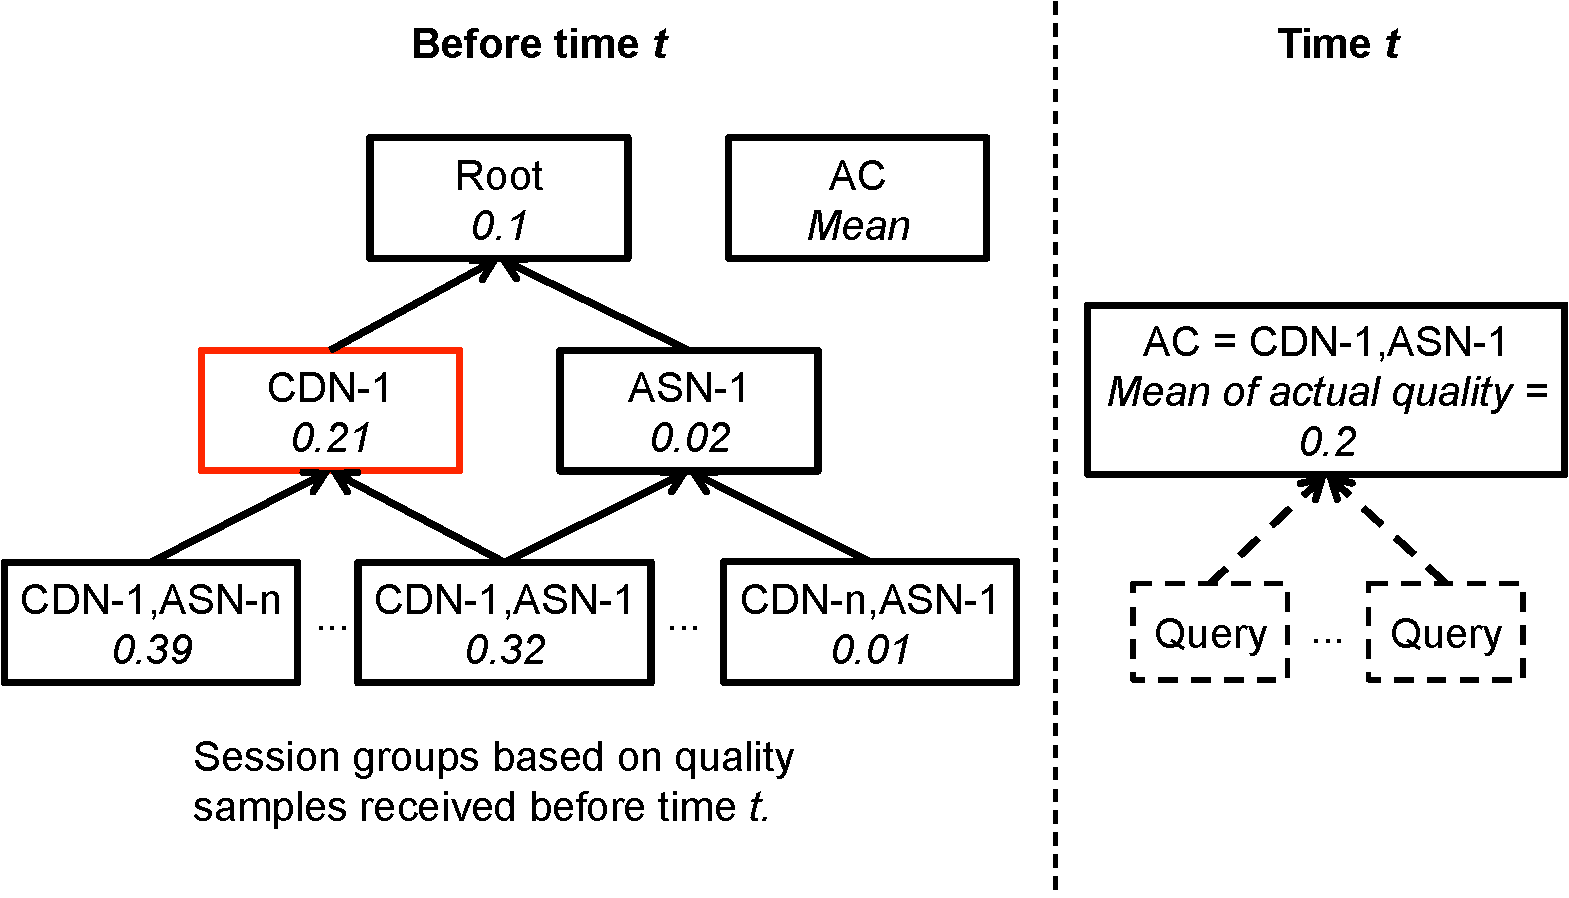
\includegraphics[width=0.5\textwidth] {figures/fig-optimal-AC.pdf}
\tightcaption{Example of how optimal AC is identified. The optimal AC is colored in red. The optimal AC  is the one minimizing the prediction error.}
\label{fig:example-optimal-ac}
\end{figure}

\myparatight{Optimal AC} To illustrate the impact of the aggregation
granularity on the prediction accuracy, we use an oracle methodology,
called {\it optimal AC}. This methodology aims to determine the
optimal AC for each session $s$, that is, the AC which provides the
best prediction quality for $s$.

Recall that given an AC, any prediction algorithm provides the same
predicted quality for all sessions in the same AC partition (i.e., it
cannot dscrimnate between two sessions in the same partition), and
that the prediction error is minimized when the predicted quality for
a partition is the mean of the actual quality values over all sessions
in that partition.

To illustrate this methodoly, consider session $s$ at time $t$, where
$s$ is identified by attributes $[CDN$-$1, ASN$-$1, Site$-$1]$ and has
an actual quality at time $t$ of $0.2$. Then, the optimal AC for this
session is the AC whose predited quality to $s$ (based on the
information collected \emph{before} time $t$) is the closest to the
actual quality of $s$ at time $t$.  In particular,
Figure~\ref{fig:example-optimal-ac} shows all possible partitions that
match at least one of the attributes of session $s$. In this case, the
partition with the predicted quality closest to the actual quality of
$s$ is the partition defined by attribute values $[CDN$-$1, Site$-$1]$
(shown by the red rectangle), i.e., the predicted quality is $0.21$
while the actual quality is $0.2$. Thus, the optimal AC for $s$ is
$[CDN, Site]$.

\comment{
Figure~\ref{fig:example-optimal-ac} shows all possible ACs
where each layer corresponds to a given level of aggregation, i.e.,
ACs with one attribute, ACs with two attributes, and so on.

an example of optimal AC
with three attributes. For the finest granularity partition (e.g.,
$[CDN1,ASN1,Site1]$) at $t$-th minute, we first build a hierarchy,
where each layer corresponds to a particular aggregation level: no
aggregation, aggregation by one attribute, aggregation by two
attributes, and full aggregation (e.g., see left hand side of
Figure~\ref{fig:example-optimal-ac}).  Remember that the optimal
prediction of a given partition is the mean of the actual quality
across all sessions in that partition (see
\Section~\ref{subsec:lowerbound}).
% Then, the optimal AC for this partition is the degree of
% aggregation that corresponds to the
% prediction value closest to the optimal prediction for the finest
% partition at $t$-th minute.  
For instance, in Figure~\ref{fig:example-optimal-ac}, if the optimal
prediction of the targeted partition is 0.2, the optimal AC (colored
in red) is the one with the closest prediction to 0.2, i.e., $(ASN,
CDN)$.
}

Note that no practical algorithm can compute the optimal AC as this
requires an oracle that knows the quality information of every session
\emph{after} the prediction takes place. However, the optimal AC
reflects the best possible predition that one can make based on the
historical data. Next, we use empirical analysis over our data sets to
evaluate the characteristics of the optimal ACs.

\begin{figure}[h!]
\centering
\subfigure[Distribution of coverage of top five optimal ACs (w.r.t averge bitrate).]
{
        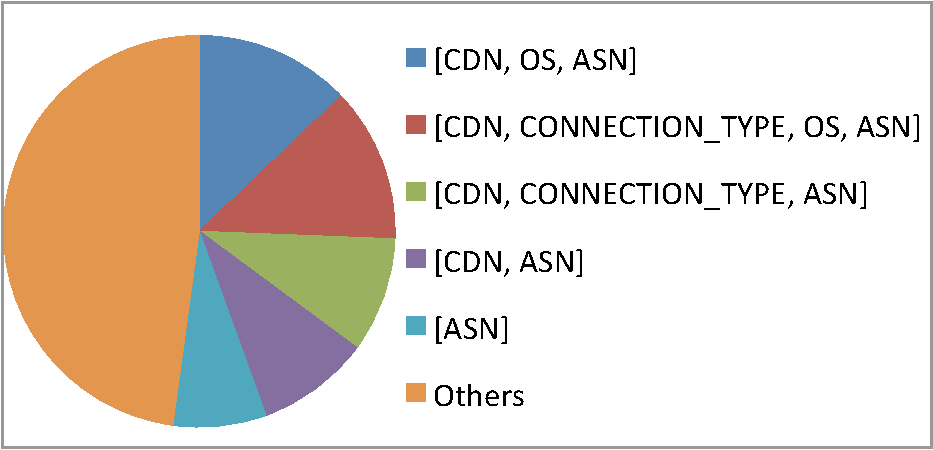
\includegraphics[width=0.4\textwidth]{figures/optimal_AC_distribution.pdf}
}
\subfigure[Optimal AC prevalence.]
{
        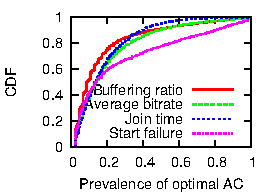
\includegraphics[width=0.24\textwidth]{figures/optimal-prevalence.pdf}
}
\hspace{-0.6cm}
\subfigure[Optimal AC persistence.]
{
        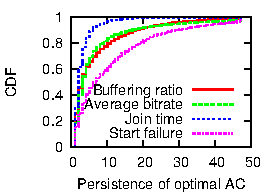
\includegraphics[width=0.24\textwidth]{figures/optimal-persistence.pdf}
}
\tightcaption{Dynamics of the optimal AC. (a) the coverage of optimal ACs (for each AC, the fraction of sessions for which this AC is the optimal AC). (b) the prevalence of the (session under prediction, optimal AC) tuples (the fraction of time that the finest granularity AC corresponds to the optimal AC). (c) the persistence of the (session under prediction, optimal AC) tuple (i.e., the longest continuous duration where a finest granularity AC corresponds to the optimal AC).}
\label{fig:optimal-ac-dynamics}
\end{figure}


 
\begin{packeditemize}
	\item {\it No single optimal AC:} Figure~\ref{fig:optimal-ac-dynamics}-(a) shows the coverage of different optimal ACs, i.e., the fraction of sessions under prediction for which a given AC is its optimal one. Note that there is no single optimal AC that covers most sessions. For example, the finest granularity AC covers only about 20\% of all sessions, and no single attribute AC is among the top 5 in terms of coverage. 
%This implies that the optimal ACs are often in between.
	\item {\it No temporally prevalent optimal AC:} Figure~\ref{fig:optimal-ac-dynamics}-(b) shows the session-level prevalence of an optimal AC, i.e., the fraction of time a session has the same AC as its optimal AC. Note that $70\%$ of (session, optimal AC) pairs only last for less than $20\%$ of time. This implies that there is no single or a small set of optimal ACs that can cover most of sessions.
	\item {\it Highly dynamic optimal ACs:} Figure~\ref{fig:optimal-ac-dynamics}-(c) shows the session-level persistence an optimal AC, i.e., the longest continuous duration where a session under prediction has the same optimal AC. Only 40\% of (session, optimal AC) tuples last for more than 10 minutes. This suggests that even with a reactive strategy it will be challenging to dynamically track the optimal ACs.
\end{packeditemize}

To conclude, we find that the optimal AC (the aggregation that gives minimal prediction error) is in many cases neither the finest nor the coarsest one, and, in addition, is highly dynamic. This makes the designing of a practical prediction algorithm highly challenging.


